%%%%%%%%%%%%%%%%%%%%%%%%%%%%%%%%%%%%%%%%%%%%%%%%
% E.Pinault-Bigeard - e.pinault-bigeard@upsti.fr
% http://s2i.pinault-bigeard.com
% CC BY-NC-SA 2.0 FR - http://creativecommons.org/licenses/by-nc-sa/2.0/fr/
%%%%%%%%%%%%%%%%%%%%%%%%%%%%%%%%%%%%%%%%%%%%%%%%
\documentclass[11pt, multicol]{article}
%%%%%%%%%%%%%%%%%%%%%%%%%%%%%%%%%%%%%%%%%%%%%%%%
% Package UPSTI_Document
%%%%%%%%%%%%%%%%%%%%%%%%%%%%%%%%%%%%%%%%%%%%%%%%
%%%%%%%%%%%%%%%%%%%%%%%%%%%%%%%%%%%%%%%%%%%%%%%%
% Package UPSTI_Document
%%%%%%%%%%%%%%%%%%%%%%%%%%%%%%%%%%%%%%%%%%%%%%%%
\usepackage{subcaption}
\usepackage[usenames, svgnames, dvipsnames]{xcolor}
\usepackage{UPSTI_Document}
\usepackage{pgfplots}
\usepackage{import}
\definecolor{darkspringgreen}{rgb}{0.09, 0.45, 0.27}

\newcommandx*{\dessinRepereFigGeo}[5][1=\vx{},2=\vy{},3=\vz{},4=,5=0]
	{
		\draw [->,very thick] (0,0) -- (1,0) ;
		\draw [->,very thick] (0,0) -- (0,1) ;
    \fill[white] (0,0) circle (0.13);
    \draw [->,very thick] (0,0) circle (0.13);
    \ifnumequal{#5}{0} {% z vers nous
      \fill[black] (0,0) circle (0.03);
      \draw [->,thick] (0,0) circle (0.04);
    }{% z vers la feuille
  		\begin{scope} [rotate=45]
  			\draw [-,thick] (0,-0.12) -- (0,0.12) ;
  			\draw [-,thick] (-0.12,0) -- (0.12,0) ;
  		\end{scope}
    }
		\draw [anchor=north west] (1.1,0) node {${#1}$};
		\draw [anchor=south west] (0,1.1) node {${#2}$};
		\draw [anchor=north east] (-0.1,0) node {${#3}$};
		\draw [anchor=north west] (-0.1,-0.1) node {${#4}$};
	}

	\usepackage{array}
	\newcolumntype{L}[1]{>{\raggedright\let\newline\\\arraybackslash\hspace{0pt}}m{#1}}
	\newcolumntype{C}[1]{>{\centering\let\newline\\\arraybackslash\hspace{0pt}}m{#1}}
	\newcolumntype{R}[1]{>{\raggedleft\let\newline\\\arraybackslash\hspace{0pt}}m{#1}}

	\usepackage{pifont}% http://ctan.org/pkg/pifont
\newcommand{\cmark}{\color{green}\ding{51}}%
\newcommand{\xmark}{\color{red}\ding{55}}%
\newcommand{\fmark}{\ding{229}}%
\newcommand{\itemc}{\item[\cmark]}%
\newcommand{\itemx}{\item[\xmark]}%
\newcommand{\itemf}{\item[\fmark]}%

\usepackage{multirow}
%---------------------------------%
% Paramètres du package
%---------------------------------%

% Version du document (pour la compilation)
% 1: Document prof
% 2: Document élève
% 3: Document à publier
\newcommand{\UPSTIidVersionDocument}{2}


% Classe
% 1: PTSI				6: PSI*			11: TSI2		16: Spé
% 2: PT	(par défaut)	7: MPSI			12: ATS
% 3: PT*				8: MP			13: PC
% 4: PCSI				9: MP*			14: PC*
% 5: PSI				10: TSI1		15: Sup
%\newcommand{\UPSTIidClasse}{2}



% Matière
% 1: S2I (par défaut)    2: IPT     3: TIPE
% 6: Vie au lycée
\newcommand{\UPSTIvariante}{5}
\newcommand{\UPSTIidMatiere}{0}
\newcommand{\UPSTIintituleMatiere}{Automatique}
\newcommand{\UPSTIsigleMatiere}{Autom}
% Type de document
% 0: Custom*				7: Fiche Métho de			14: Document Réponses
% 1: Cours (par défaut)		8: Fiche Synthèse    		15: Programme de colle
% 2: TD     				9: Formulaire
% 3: TP						10: Memo
% 4: Colle					11: Dossier Technique
% 5: DS						12: Dossier Ressource
% 6: DM						13: Concours Blanc
% * Si on met la valeur 0, il faut décommenter la ligne suivante:
%\newcommand{\UPSTItypeDocument}{Custom}
\newcommand{\UPSTIidTypeDocument}{1}

% Titre dans l'en-tête


% Titre dans l'en-tête

\newcommand{\UPSTIvariante}{5}

\newcommand{\UPSTItitreEnTete}{Automatisme industriel}
%\newcommand{\UPSTItitreEnTetePages}{}
\newcommand{\UPSTIsousTitreEnTete}{Introduction aux API}


% Titre
%\newcommand{\UPSTItitrePreambule}{Automatisme industriel}
\newcommand{\UPSTItitre}{La programmation d'un Automate Industriel}

% Durée de l'activité (pour DS, DM et TP)
\newcommand{\UPSTIduree}{3h30}

% Note de bas de première page
%\newcommand{\UPSTInoteBasDePremierePage}{Geoffrey Vaquette}
% Numéro (ajoute " n°1" après DS ou DM)
\newcommand{\UPSTInumero}{2}

% Numéro chapitre
%\newcommand{\UPSTInumeroChapitre}{1}

% En-tête customisé
%\newcommand{\UPSTIenTetePrincipalCustom}{UPSTIenTetePrincipalCustom}

% Message sous le titre
%\newcommand{\UPSTImessage}{Message sous le titre}


% Référence au programme
%\newcommand{\UPSTIprogramme}{\EPBComp \EPBCompP{B1-02}, \EPBCompP{B2-49}, \EPBCompS{B2-50}, \EPBCompS{B2-51}, \EPBCompP{C1-07}, \EPBCompP{C1-08}}

% Si l'auteur n'est pas l'auteur par défaut
%\renewcommand{\UPSTIauteur}{WWOOOOOOWW}

% Si le document est réalisé au nom de l'équipe
%\newcommand{\UPSTIdocumentCollegial}{1}

% Source
\newcommand{\UPSTIsource}{G. Vaquette, A. Juton, J. Deprez, J. Maillefert}

% Version du document
\newcommand{\UPSTInumeroVersion}{1}

%-----------------------------------------------
\UPSTIcompileVars		% "Compile" les variables
%%%%%%%%%%%%%%%%%%%%%%%%%%%%%%%%%%%%%%%%%%%%%%%%


%%%%%%%%%%%%%%%%%%%%%%%%%%%%%%%%%%%%%%%%%%%%%%%%
% Début du document
%%%%%%%%%%%%%%%%%%%%%%%%%%%%%%%%%%%%%%%%%%%%%%%%
\newcommand{\nomTP}{triDePiece}
\begin{document}
\UPSTIbuildPage
\UPSTIobjectif{\begin{itemize}
	\item Reconnaissance de la partie opérative
	\item Identification des capteurs et des actionneurs
 	\item Identification des éléments de la commande
	\item Prise en main de l’outil de développement
 	\item Mise au point de programmes de test
\end{itemize}}

\tableofcontents


\section{Introduction}
\begin{figure}[ht]
	\centering
	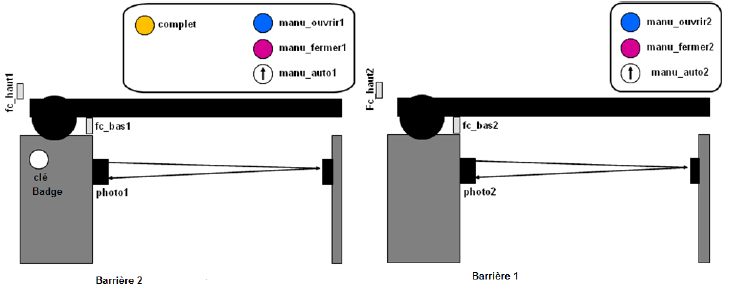
\includegraphics[width=.63\linewidth]{images/schemaSysteme}
	\caption{Partie opérative du système de tri de pièce}
	\label{fig:schemaPartieOperative}
\end{figure}
Dans ce TP, on met en oeuvre une charge opérative modélisant un tri de pièces selon leur hauteur (Figure~\ref{fig:schemaPartieOperative}). Ce système est piloté par un automate programmable MODICON de la marque SCHNEIDER. On fera, dans un premier temps, un test des capteurs et des actionneurs.
On prendra en main, à cette occasion, l’outil de développement \textbf{EcoStruxure} de \textit{Schneider Electric} pour l’automate. On écrira pour finir une application sous forme d’un GRAFCET, que l’on testera.

\section{Partie opérative}
\subsection{Description}
L’appareil est destiné à trier des pièces métalliques suivant leur hauteur. En fonction de la hauteur, les pièces acheminées par le convoyeur sont éjectées dans le bac 1, le bac 2, le bac 3 ou continuent leur trajet sur le convoyeur (Figure~\ref{fig:schemaPartieOperative}). La liste des différents capteurs et actionneurs est données dans le Tableau~\ref{tab:capteursActionneurs}.

\begin{table}[ht]
\centering
	\begin{tabular}{|ll || ll|}
	\hline
		\multicolumn{2}{|c||}{Capteurs}       				& \multicolumn{2}{c|}{Actionneurs}                  \\\hline
		\multirow{5}{*}{Capteurs fin de course}  & capt\_S\_V1    & \multirow{5}{*}{Vérins pneumatiques} & V1 \\
		                                         & capt\_S\_V2    &                                      & V2 \\
		                                         & capt\_S\_V3    &                                      & V3 \\
																						 & capt\_S\_VB		&                                      & VB \\
																						 & capt\_S\_VTR   &                                      & VTR\\\hline
		\multirow{3}{*}{Capteurs inductifs}      & DPI1         & Moteur convoyeur                     & MC \\\cline{3-4}
		                                         & DPI2         &                                      &    \\
		                                         & DPI3         &                                      &    \\\hline
	\end{tabular}
	\caption{Liste des capteurs et actionneurs}
	\label{tab:capteursActionneurs}
\end{table}
\paragraph{Approvisionnement en pièces : } Les pièces sont acheminées vers le convoyeur par une goulotte inclinée. Le vérin \textbf{simple effet}
VB bloque la pièce au bas de la goulotte. Il faut rentrer le vérin pour libérer la pièce.

\paragraph{Mesure de la hauteur des pièces : }La mesure de la hauteur des pièces est effectuée par via le capteur situé au pied de la goulotte d’approvisionnement. Celui-ci, via des convertisseurs analogique/numérique, délivre 3 signaux pièce1, pièce2, pièce3 selon la table de vérité du Tableau~\ref{tab:hauteurPiece}
\begin{table}[ht]
	\centering
	\begin{tabular}{lccc}
		\textbf{Type de pièce} & \textbf{Piece3} & \textbf{Piece2} & \textbf{Piece1}\\
		Absence de pièce       & 0               & 0               & 0              \\
		Petite (\SI{20}{mm}) 	 & 0               & 0               & 1              \\
		Moyenne (\SI{22}{mm})  & 0               & 1               & 1              \\
		Grande (\SI{25}{mm})   & 1               & 1               & 1              \\
	\end{tabular}
	\caption{Mesure de hauteur de pièce}
	\label{tab:hauteurPiece}
\end{table}




\paragraph{Transfert sur le convoyeur : } Le transfert des pièces de la goulotte sur le convoyeur est assuré par le vérin simple effet VTR.

\paragraph{Déplacement par convoyeur : } Le convoyeur est entraîné à vitesse constante par un moteur électrique asynchrone MC. Ce dernier est piloté via un contacteur (relais de puissance).
Un réducteur mécanique adapte la vitesse. Le moteur, est piloté par l’automate via un contacteur (relais de

\paragraph{Ejection des pièces dans les bacs : } Les vérins \textbf{simple effet} V1, V2 et V3 éjectent les pièces depuis le convoyeur vers les bac 1, 2 et 3 respectivement.

\paragraph{Détection des pièces non triées : } Les pièces non triées sont acheminées vers l’extrémité du convoyeur. Un capteur indique
quand une pièce dépasse cette extrémité.

\subsection{A propos des actionneurs pneumatiques}
Le montage comporte des actionneurs électriques (comme le moteur) et pneumatiques (les vérins).
La commande de ces actionneurs pneumatiques (vérins simple effet) se fait par l’intermédiaire
d’électro distributeurs (vannes pneumatiques commandées électriquement).

Lorsqu'une tension de 24V est appliquée à la bobine des électro distributeurs, elle provoque la commutation des circuits d’air. L'air comprimé augmente alors la pression d'un côté du corps du vérin associé provoquant la sortie (ou retour) de la tige du vérins.
Pour chacun de ces verins, des capteurs permettent de tester leur état « SORTI » (repérés B5, B6, B7, B8, B9 sur la maquette).

\UPSTIattention{Il faut vérifier que le compresseur de la salle de TP a été mis en marche.}

\section{Partie commande (API)}
La partie commande est assurée par un automate \textit{MODICON} du constructeur \textit{Schneider}. Il dispose d'un module d'entrée TOR et d'un module de sortie TOR.

\UPSTIrappel{\begin{itemize}
	\item Les \textbf{capteurs} de la partie opérative sont reliées aux \textbf{entrées} de l'automate.
	\item Les \textbf{actionneurs} de la partie opérative sont reliées aux \textbf{sorties} de l'automate.
\end{itemize}
}
\subsection{Table d'entrée-sortie de l'automate}
Afin de gagner du temps lors du TP, nous fournissons un projet configuré à l'avance. La table des entrées-sorties est incluse à ce projet (Figure~\ref{fig:entreesSorties})
\begin{figure}
	\centering
	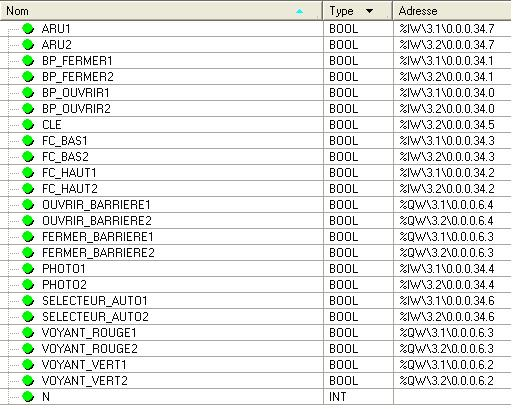
\includegraphics[width=.9\textwidth]{images/listeES}
	\caption{Table des entrées et sorties au sein du projet}
	\label{fig:entreesSorties}
\end{figure}
\pagebreak
\section{Travail demandé}
\subsection{Mise en place informatique}
\begin{UPSTIactivite}[3][Structure du répertoire]
	Dans votre dossier personnel,
	\begin{enumerate}
		\item Créer un dossier intitulé TP03-\nomTP (ou TP04-\nomTP)
		\item Dans ce dossier, créer un dossier \textit{compte-rendu}
		\begin{itemize}
			\item Il contiendra les images, données et le compte-rendu en lui-même
		\end{itemize}
		\item Créer un dossier \textit{projetEcostruxure}
		\item Y copier le contenu du dossier \textit{\nomTP} fourni sur \textit{Commun/Automatisme\_et\_distribution}

	Une fois votre dossier configuré, nous allons compiler et envoyer le projet sur l'automate pour vérifier que la communication entre le PC et l'automate est fonctionnelle.

		\item Ouvrir le projet à l'aide du logiciel \textit{EcoStruxure}
		\item Mettre l'automate sous tension puis compiler et transférer le programme.
		\item Lancer le programme sur l'automate (\textbf{Exécuter})
	\end{enumerate}
\end{UPSTIactivite}
\subsection{Consignes et conseils pour la rédaction du compte-rendu}
Vous rédigerez un compte-rendu détaillé des manipulations effectuées celui du TP 3 servira d'entraînement et comptera avec un coefficient moins important que celui du TP4.

\UPSTIremarque{
Le compte-rendu évalue votre capacité à \textbf{expliquer et synthétiser} votre démarche et les manipulations effectuées.
Les manipulations en elle-même sont observées durant la séance par l'enseignant.}

Vous pourrez donc insérer des captures d'écrans, photos et tout schéma pouvant aider à la compréhension de votre propos.
Un bon compte-rendu est un compte-rendu \textbf{lisible et entièrement compréhensible} par une personne n'ayant pas participé au TP et ayant un niveau de connaissance similaire au vôtre.


\subsection{Prise en main et vérification du fonctionnement du système}
La première chose à vérifier avant d'entreprendre la programmation d'un automate est de vérifier le bon fonctionnement des entrées et sorties de l'automate.
\begin{UPSTIactivite}[][Test des capteurs]
	Avec l'automate sous tension, vérifier \textbf{un à un} le bon fonctionnement de \textbf{tous les capteurs} en vérifiant que la LED correspondante sur le module d'entrées s'allume ainsi que le changement d'état dans la table d'animation du projet.

	Si un capteur ne fonctionne pas ou que son état ne varie pas dans la table d'animation, chercher alors la cause de ce disfonctionnement.
\end{UPSTIactivite}
\UPSTIboiteGenerique{Aide à la rédaction}{\bcplume}{
A titre d'exemple, pour la présentation des tests des capteurs dans votre compte-rendu, vous pouvez expliquer la démarche générale puis insérer une capture d'écran du test d'un des capteurs avec l'explication associée. Il n'est pas alors nécessaire de faire une capture pour chaque capteur.

Décrivez également tout disfonctionnement rencontré et comment il a été corrigé.}

\begin{UPSTIactivite}[][Test des actionneurs]
Pour tester les actionneurs, il est nécessaire de commander les sorties de l’automate. Pour cela, le capot de protection doit être fermé.

Dans la table d'animation, cliquer sur \textit{Modifications} afin d'activer la commande des sorties.

Vérifier \textbf{un à un} le bon fonctionnement de \textbf{tous les actionneurs} en vérifiant que la LED correspondante sur le module de sortie s'allume et que l'actionneur s'active.
\end{UPSTIactivite}

\subsection{Programmation de l'automate}
\subsubsection{Ejection des pièces dans le premier bac}
On propose le cahier des charges suivant :
\UPSTIboiteGenerique{Cahier des charges 1 : Transfert dans le premier bac.}{\bcoutil}{
\begin{itemize}
	\item Les pièces sont introduites par l'utilisateur dans la goulotte d'approvisionnement \textit{une par une}. Le vérin bloqueur n'est donc pas utilisé.
	\item Les pièces sont toutes transférées sur le tapis puis dans le bac 1.
\end{itemize}}

\begin{UPSTIactivite}[][Implémentation du Cahier des charges 1]
	\begin{enumerate}
		\item Dessiner sur papier ou à l'aide d'un logiciel adapté le GRAFCET à implémenter (il a normalement été vu en TD)
		\item Créer une section dans le projet et implémenter la structure du GRAFCET
		\item Ajouter un commentaire à côté de chage action pour décrire les actions voulues
		\item Implémenter les transitions (penser à créer des sections transitions au besoin, donner des noms \textbf{compréhensibles})
		\item Ajouter et implémenter une section transitions (LADDER ou ST) pour l'activation des actionneurs
	\end{enumerate}
\end{UPSTIactivite}
\UPSTIboiteGenerique{Aide à la rédaction}{\bcplume}{
	A titre d'exemple, dans votre compte-rendu, vous pouvez insérer le GRAFCET ainsi que la section actionneurs. Vous pouvez également expliquer la démarche pour construire un des réseaux du programme LADDER.
}

\begin{UPSTIactivite}[][Ajout d'un compteur]
	Ajouter un compteur permettant de connaitre le nombre de pièces éjectées dans le bac.
	\begin{enumerate}
		\item Dessiner les modifications
		\item Les implémenter
	\end{enumerate}
\end{UPSTIactivite}

\UPSTIpresenceProf[Faire vérifier le bon fonctionnement]{S'il nest pas disponible, sauvegarder cette version et continuer le TP en attendant.}

\subsubsection{Tri des pièces}
\UPSTIboiteGenerique{Cahier des charges 2 : Transfert dans le premier bac.}{\bcoutil}{
\begin{itemize}
	\item Une ou plusieurs pièces sont introduites par l'utilisateur dans la goulotte d'approvisionnement.
	\item Le vérin VB bloque les pièces avant le capteur entre chaque tri
	\item Les pièces sont transférées sur le tapis puis triées :
	\begin{itemize}
		\item Les petites pièces sont éjectées dans le bac 1
		\item Les pièces de taille moyenne sont éjectées dans le bac 2
		\item Les grandes pièces sont éjectées dans le bac 3
	\end{itemize}
	\item Une fois que la pièce a été éjectée dans son bac, le vérin VB laisse la pièce suivante passer puis elle est triée à son tour.
\end{itemize}}

\begin{UPSTIactivite}[][Implémentation du tri de pièce]
	Implémenter le comportement du cahier des charges 2 puis vérifier le bon fonctionnement.
\end{UPSTIactivite}
\UPSTIboiteGenerique{Aide à la rédaction}{\bcplume}{
	A titre d'exemple, vous pouvez expliquer les éventuelles divergences et les choix qui ont été faits pour ce comportement.

	Il est encore une fois pertinent d'insérer quelques captures et d'expliquer votre démarche.
}
\begin{UPSTIactivite}[2][Pour aller plus loin]
	Ajouter un compteur pour chacun des bacs
\end{UPSTIactivite}
\begin{UPSTIactivite}[2][Pour aller encore plus loin -- difficile]
	Ne plus attendre qu'une pièce soit éjectée dans un bac pour envoyer la suivante sur le tapis.
\end{UPSTIactivite}


\end{document}
